\documentclass{article}
\usepackage[utf8]{inputenc}
\usepackage{mathtools}
\usepackage{tikz}
\usetikzlibrary{arrows,positioning,shapes.geometric}

\title{ArenaPeds: Pedestrian Flow in a highly crowded stadium}
\author{Jan Erik van Woerden}
\date{The end of September 2020}

\begin{document}

\maketitle

\section{Introduction}
In a world with increasing accessibility to information, it is important to summarize this information into useful information for the users.  In this case we have access to a huge amount of surveillance camera's which are used during busy events. To monitor all these camera's it requires a lot of manual watching what is happening on those camera's. There has a lot of research been done on reducing the amount of manual watching and translating the information into more actionable and measurable tasks.

The research can be ranging from quite low level to more high level. On a low level we have Crowd Counting which is to measure how how many individuals are present in an certain frame. As well as which direction a person is going, Crowd Direction. On a mid level we try to extract information over a time frame of the frame, Line of Interest is a good example of this. With Line of Interest the goal is to count how many people crossed the line in a time frame. An example of this is counting how many people went inside a stadium and went out. Lastly on a high level we want to make decisions based on both these high and mid level information, such as finding jam's inside a crowd.

In this thesis we will mostly focus on Line of Interest. Line of Interest is an area which hasn't had a lot of improvements since 2016, but there were still a lot improvements around the building blocks of LOI. Which is an excelent reason to check again the current LOI state-of-the-art and try to find ways to improve the SOTA with more up to date methods.

In the newer methods which we will be focusing on, there are two main components for Line of Interest. Which is Crowd Counting and Crowd Direction. Combining these two provides a estimation who crossed the line and who didn't.

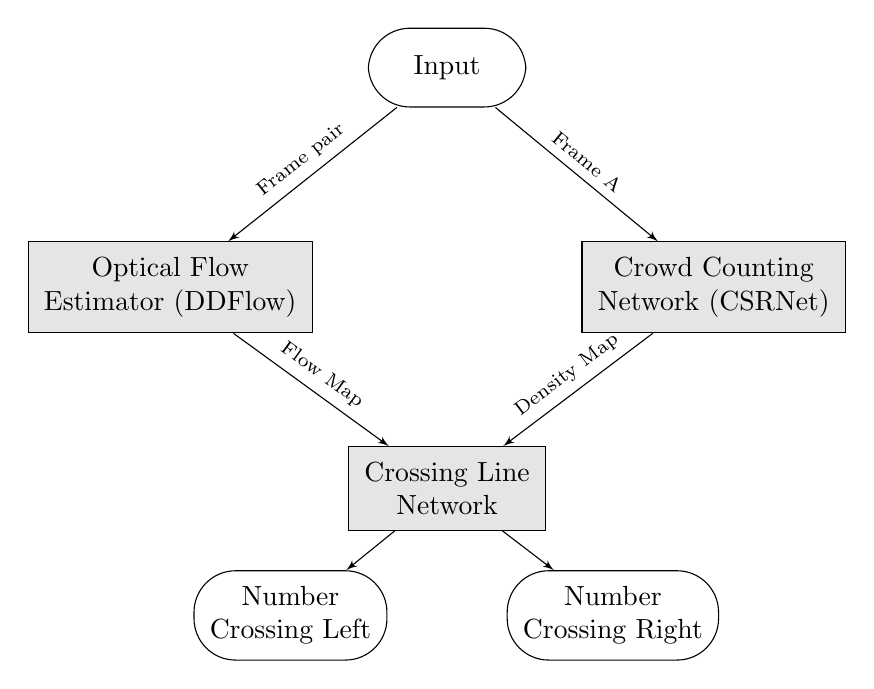
\begin{tikzpicture}[>=latex']
    \tikzset{block/.style= {draw, rectangle, align=center,minimum width=2cm,minimum height=1cm, inner sep=0.2cm, fill=gray!20},
    rblock/.style={draw, shape=rectangle,rounded corners=1.5em,align=center,minimum width=2cm,minimum height=1cm, inner sep=0.2cm},
    }
    \node [rblock]  (start) {Input};
    \node [block, below right =1.7cm and 0.7cm of start] (countnet) {Crowd Counting\\Network (CSRNet)};
    \node [block, below left = 1.7cm and 0.7cm of start] (flownet) {Optical Flow\\Estimator (DDFlow)};
    \node [block, below = 4.3cm of start] (linenet) {Crossing Line\\Network};
    \node [rblock, below right =0.5cm and -0.5cm of linenet] (crossright) {Number\\Crossing Right};
    \node [rblock, below left = 0.5cm and -0.5cm of linenet] (crossleft) {Number\\Crossing Left};
    %% Coordinate on left and middle

% paths
    \path[draw,->, every node/.style={sloped,anchor=south,auto=false, font=\scriptsize}]
                (start) edge node {Frame A} (countnet)
                (start) edge node {Frame pair} (flownet)
                (countnet) edge node {Density Map} (linenet)
                (flownet) edge node {Flow Map} (linenet)
                (linenet) edge (crossright)
                (linenet) edge (crossleft)
                ;
\end{tikzpicture}

\subsubsection{Why unsupervised}
For Crowd Counting there are a lot of datasets available and if new data is provided, it is pretty easy to label these and update the model. For Crowd Direction this is a bit more tricky. Older methods use conventional methods which used handcrafted features which predicted pretty well the direction in situations which were pretty standard, but completely failed in situations which were different from the standard. With the introduction of convolutional neural networks in the field this changed. These made it possible to make vastly more robust filters, but with cost of requiring a lot of labeled data (Because supervised learning). All approaches in the earlier papers had the access to huge amount of labeled data, which made this a suitable solution. In situations with not a lot of available data this makes it a lot harder.
The supervised models for Crowd Direction are largely based on general Flow Estimation models which try to predict all the pixels in a frame. More recently there appear methods to make the supervised Flow Estimation models unsupervised. This makes it possible to accurately predict the direction of pixels without the need for huge amounts of labeled data.

\section{Related Work}
In the following parts we try to explain several key subjects to understand the field of Line of Interest.


\subsection{Line of Interest}
In the earlier days of Line of Interest the method to estimate was by temporal slicing. In each frame a slice of the image is taken, by taking a slice around the LOI. These slices are stitched together, so a small sequence of frames result in a single image of the stitched slices, temporal slice image. Based on the image the algorithms try to predict how many pedestrians passed the line in the short sequence.

Ma et al. \cite{ma_counting_2016} first uses crowd segmentation on the sliced image, which results in several crowd segments in the image. Then the algorithm performs normalization on the pedestrians, because of the slicing the faster walking pedestrians appear smaller in the temporal slice image. After this the algorithm performs feature extraction using both global features and local features, which are extracted using local HOG (Histogram of Oriented Gradient) features and a bag-of-words model. This results in a single feature vector per crowd segment. Using a regression function with the features as input, the size of the crowd is predicted. The total pedestrian count of the sliced image is then used to calculate the exact count of people crossing the line between two individual frames. This is done by using several sliced images and solving the problem as a integer programming problem.

During the same time Cao et al. \cite{cao_large_2015} first introduced CNN's in the field of LOI. The paper proposes a model which uses three CNN's which predicts the ins and outs of a individual temporal slice. The first CNN predicts the total amount of people in the temporal slice. The second CNN classifies from which direction people are crossing the line based on the optical flow of the temporal sliced image. The third one predict the ratio of pedestrians crossing during the slice, based on the optical flow. By using the outputs of each network, the algorithm is able to accurately predict the instant count. Additionally Cao et al. \cite{cao_large_2015} shows that the use of CNN's improves the versatility of the models. The model performs better on almost all scenario's and is much more robust with changing weather scenario's and changing angles, than the method of Ma et al. \cite{ma_counting_2016}

Zhao et al. \cite{leibe_crossing-line_2016} introduced a new approach to process the images. Instead of using temporal sliced images. The method directly tries to predict the crowd count based on two consecutive frames. Additionally it merges the Crowd Counting and Crowd Flow models into a single CNN. The paper uses FlowNet as base for the model. Only the last layer predicts both the flow and the crowd density map, as described in Crowd Counting. Additionally the model doesn't try to predict precise direction of every pixel, because the labeled data provided for the model doesn't use pixel precise Flow Estimation. The flow estimator only uses the dot-annotated location of the heads.

Zheng et al. \cite{zheng_cross-line_2019} provides in a era where CNN's have most of the records in hand, a method which scores SOTA on the benchmark for LOI. The model is extremely fast and only uses SVM's and linear regression to end state of the art. Problem with the model, it is very hard to tweak to very dynamic datasets such as the ArenaPeds dataset.



- Explain quickly why we can't just use YOLO (Low density)
-

\subsection{Region of Interest}
One of the building blocks of all the information reduction is Crowd Counting/Region of Interest. In low density area's individual object detection, such as YOLO, is a good solution. In high density area's the occlusion by pedestrians makes it hard to detect individual pedestrians. Density Maps still provide the possibility to count the amount of people inside an area, but don't have to deal with the exact locations of the heads, which makes it more robust against errors in the prediction.

In contrast to object detection, it is not possible to identify the full body of the pedestrian in the frames. When using downwards facing camera's, such as high hanging surveillance camera's, the only clearly visible part of a pedestrian is the head. Therefore the labeling of the pedestrians is done by selecting a single point on the head.

An individual point is very hard for a Neural Network to find correctly and is prone to errors. Additionally the exact location of an individual pedestrian are not of high importance, only the total count given a certain region.

Density Maps for Crowd Counting are therefore a solution. Instead of finding individual points in the image, which represent a pedestrian, the points are spread out on the density map, by a Gaussian Distribution, which summed together add up to one.

This method results in a robust method to train an end-to-end model for ROI especially in high density images.

% Show a density map with on the left side a image with dots and on the right side the density map.

The density map is always a area with several Gaussians. The method to generate those Gaussian's and their size differ.

- All Gaussians same size
- Gaussians differ in size depending on the density of the pedestrians in the neighbourhood
- Gaussian differs in size based on the angle of the video. Hard to do when there is no access to height/angle.

Good paper to cite for benchmark and why we chose this method
\cite{wang2020nwpu}
\cite{li2018csrnet}



\subsection{Flow Estimation}
Since the early days of image detection different flow estimation methods are proposed. These methods are very general and can be applied to solve a range of different problems.

One of the most widely used methods is the Lucas-Kanade method (For more details \cite{lucas_kan_nutshell}), which was invented in the 80s. It tries to predict the displacement of a pixel in two consecutive frames using equation (\ref{eq:lucas1}).

\begin{equation} \label{eq:lucas1}
I_x(x, y) \cdot u + I_y(x,y) \cdot v = -I_t(x,y)
\end{equation}

With equation (\ref{eq:lucas1}) the goal is to estimate $(y, v)$ which is the direction of the pixel. $I_x(x, y)$ and $I_y(x, y)$ are the derivative of the intensity in both the $x$ and $y$ direction.$I_t(x, y)$ is the difference in intensity between the two consecutive frames $(b-a)$.

The Lucas-Kanade method is an easy and efficient method to estimate moving object, but it lacks on crucial points. It only incorporates gray scale and doesn't work very well with occluded pixels. (Linear movement? Not sure if NN's assume this as well. Probably not, but doesnt matter in our case)

\subsubsection{FlowNet}
One of the first good working models for Flow Estimation using a Neural Network based architecture is FlowNet \cite{fischer_flownet_2015} and the architecture is still widely used. (FlowNetV2 \cite{ilg_flownet_2016})

The first usable Flow Estimation using an end-to-end CNN was FlowNet, which is still widely used. The network tries per-pixel prediction which direction the flow is moving. This is done using a deep CNN and at the end a refinement to enlarge the remaining volume into an prediction with the same size as the original input frames. (Upconvolving using the output of several in between stages)

Till then a big problem was the trainability of large end-to-end CNN's and there massive hunger of data. Fischer et al. fixed this by generating a massive synthetic dataset called Flying Chairs. This dataset has more than 22000 image pairs which are build up from Flickr backgrounds and in the front chairs which have move using a random affine transformation.





Several issues with FlowNet were the complete reliability on Neural Networks. Some of the tasks inside the Flow Estimator can efficiently be solved with conventional methods. PWCNet (\cite{sun_pwc-net_2018}) uses a combination of an CNN and some conventional methods. This results in a much smaller network, which results in faster training, additionally the smaller network can handle frames quicker.

One of the issues with CNN based flow estimators is the requirement for pixel level labeling per frame. This results in a huge amount of labeled data required for training. One of the solutions for these problems is the generation of synthetic data which, but these solutions do not scale well to the real world.

A solution for the huge amount of labeled data is unsupervised learning. Both DDFlow \cite{liu_ddflow_2019} and SelFlow \cite{liu_selflow_2019} introduce methods to learn from unlabeled video.

- Video Counting explained: Deep Spatio-Temporal Residual Networks for Citywide Crowd Flows Prediction

\section{Method}

\subsection{Datasets}

\subsubsection{ArenaPeds}
For this thesis we have access to a dataset of the City of Amsterdam. It has xxx amount of footage of environments with crowds ranging from 10 pedestrians in the frame to 1000 pedestrians a few hours later. Only a tiny proportion is labeled with where each pedestrian is. So there is no labeled data on the Crowd Direction, only for the Crowd Counting. This is the reason why we want to try to give unsupervised learning a shot.


\section{Implementation}

\bibliographystyle{apalike}
\bibliography{all}

\end{document}
